\documentclass[12pt, a4paper]{article}

\usepackage[T1]{fontenc}
\usepackage{graphicx}
\usepackage{setspace}
\usepackage{float}
\usepackage{amsmath, amsthm, amssymb, amsfonts}
\usepackage[left=3cm, top=3cm, right=2cm, bottom=2cm]{geometry}
\usepackage{framed}
\usepackage{indentfirst}
\usepackage{thmtools}
\usepackage[utf8]{inputenc}
\usepackage[english,brazil]{babel}
\usepackage{framed}
\usepackage[dvipsnames]{xcolor}
\usepackage{tcolorbox}
% Configurações das referências
\usepackage[nottoc,notlot,notlof]{tocbibind}
\usepackage[backend=biber,style=abnt,backref=true,backrefstyle=none]{biblatex}
\nocite{*}
\addbibresource{ref.bib}

\graphicspath{ {./img/} }
% links
\usepackage{hyperref}
\setlength{\parindent}{1.25cm}
\graphicspath{ {./} }
\begin{document}
% capa
\begin{titlepage}
\begin{center}
    \large
     {\bf Centro Estadual de Educação Tecnológica Paula Souza} \\
     {\bf Faculdade de Tecnologia Baixada Santista
Rubens Lara} \\ 
    {\bf Curso Superior de Tecnologia em Ciência de Dados} \\
    
    \vspace{215pt}
        {\bf Álgebra Linear} \\
    \vspace{10pt}
        {\Large \bf Analise de Componentes Principais (PCA)}\\
        
    \vspace{100pt}

    \vfill
        {\large  \bf Autores} \\
        {\large  \bf Enri Iwasaki} \\
        {\large  \bf Fernando Gomes Cruz} 
    \vfill
        \textbf{{\large Santos}\\
        {\large 2023}}
        
\end{center}
\end{titlepage}

\tableofcontents

\newpage

\section{Introdução}

Nesse relatório será descrita a Análise de Componentes Principais (PCA) aplicada a um conjunto de dados de informações sobre indivíduos com síndrome metabólica. O PCA é uma técnica poderosa no campo da estatística multivariada, usada para reduzir a dimensionalidade de conjuntos de dados complexos \autocite{jolliffe2016principal}. Ela busca identificar padrões e estruturas subjacentes, transformando variáveis inter-relacionadas em um conjunto menor de variáveis não correlacionadas, chamadas de componentes principais. Ao reorganizar os dados de forma a preservar a maior parte da sua variabilidade original, a PCA permite uma compreensão mais simplificada dos dados, facilitando a interpretação, visualização e análise, sendo aplicável em diversos campos, desde a análise de dados científicos até a compressão de informações em tecnologias de processamento de imagens e reconhecimento de padrões.

\section{Conjunto de Dados}

O dataset utilizado na análise foi disponibilizado em formato .csv (comma-separated values) através do kaggle 
\begin{center}
\url{ https://www.kaggle.com/datasets/antimoni/metabolic-syndrome }
\end{center} e contém informações sobre indivíduos com síndrome metabólica, uma condição médica complexa associada a um conjunto de fatores de risco para doenças cardiovasculares e diabetes tipo 2. Os dados incluem medidas demogr\'{a}ficas, clínicas e laboratoriais, bem como a presença ou ausência de síndrome metabólica. Para fácil manipulação, o dataset obtido foi renomeado para 'data.csv'.

\section{Implementação}
A implementação do algoritmo de Análise de Componentes Principais (PCA) foi codificada em Python, utilizando bibliotecas como NumPy e Pandas para manipulação eficiente de dados, Matplotlib e Axes3D para visualização gráfica, entre outros. A principal funcionalidade é implementada por meio da importação das classes PCA e StandardScaler do módulo scikit-learn.
\subsection{Visualização dos dados}
Primeiramente, os dados foram lidos com o uso da biblioteca Pandas, e gerou-se uma visualização dos primeiros elementos da tabela. A partir dessa visualização, colunas relevantes para esse trabalho foram selecionadas. 

\break

\begin{figure}[h]
    \centering
    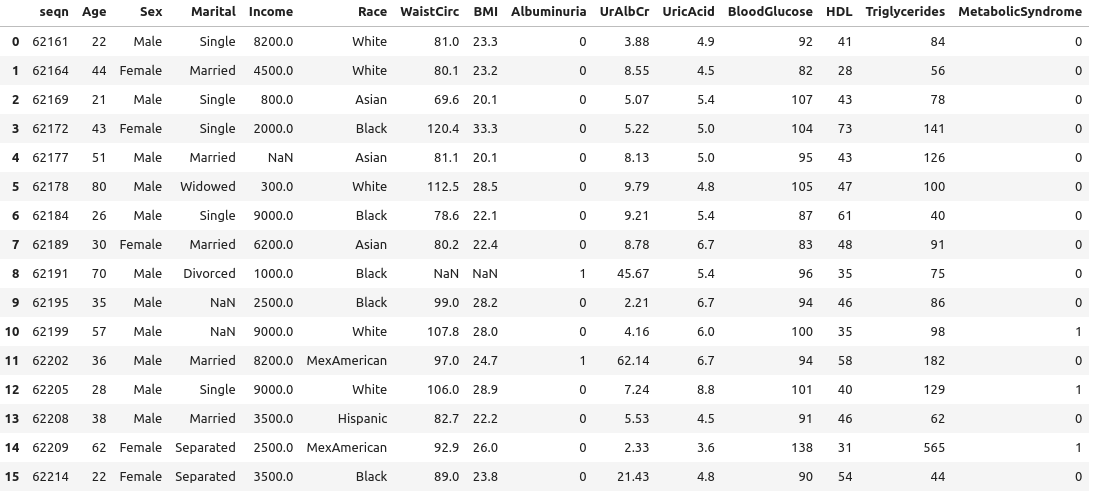
\includegraphics[scale=0.4]{img/head.png}
    \caption{Visualização das entradas de data.csv}
\end{figure}

A partir da visualização dos elementos de datasets, foram selecionadas colunas consideradas relevantes para a análise, destacando características específicas associadas ao metabolismo, como idade (Age), circunferência da cintura (WaistCirc), índice de massa corporal (BMI), albuminúria (Albuminuria), creatinina urinária de albumina (UrAlbCr), ácido úrico (UricAcid), glicose sanguínea (BloodGlucose), lipoproteína de alta densidade (HDL), e triglicerídeos (Triglycerides). A coluna alvo para a análise, relacionada à Síndrome Metabólica (MetabolicSyndrome), é especificada. \\

\subsection{Matriz de correlação e mapa de calor}
\par
Após a obtenção as colunas de interesse, realizou-se a computação  da matriz de correlação entre as variáveis presentes no conjunto de dados e a partir desta, gerou-se um mapa de calor da matriz de correlação previamente calculada, utilizando a biblioteca Seaborn. O mapa de calor é uma representação visual da matriz de correlação de acordo com os valores numéricos associados. A intensidade e a tonalidade das cores refletem a força e a direção das relações lineares entre as variáveis, proporcionando uma representação gráfica mais acessível e interpretável em comparação com a matriz de correlação tabular. 

\begin{figure}[htbp]
    \centering
    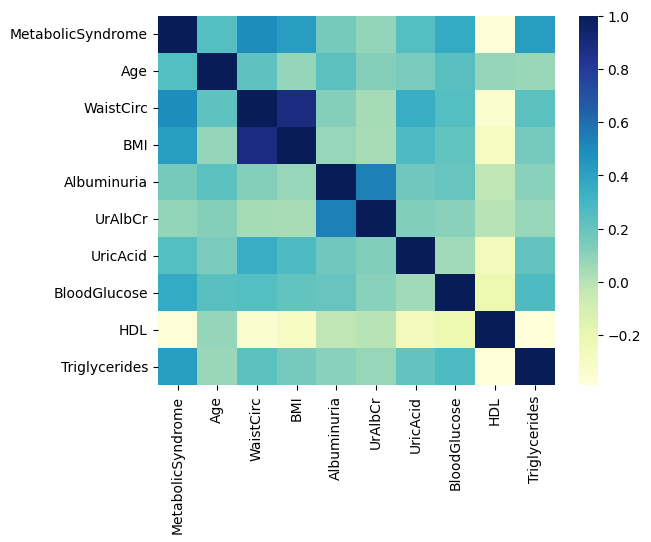
\includegraphics[scale=0.5]{img/heat.png}
    \caption{Visualização do mapa de calor da correlação.}
\end{figure}
\break
Após a preparação dos dados, e visualização do mapa de calor, ocorre a subdivisão do conjunto de dados entre as variáveis independentes (X), representadas pelas colunas numéricas previamente selecionadas, e a variável dependente (y), associada à Síndrome Metabólica.
Em seguida, procede-se à padronização das variáveis independentes (X) por meio da instância do objeto StandardScaler da biblioteca scikit-learn. A padronização é uma prática comum na preparação de dados para o PCA, garantindo que todas as variáveis tenham média zero e desvio padrão unitário. \par
\subsection{Análise de Componentes Principais}
Realiza-se a aplicação da técnica de Análise de Componentes Principais (PCA). O objeto PCA é instanciado, representado pela variável pca, e posteriormente aplicado aos dados padronizados (X\_scaled) por meio da função fit\_transform. A aplicação do PCA tem como intuito a transformação das variáveis originais em um novo conjunto de variáveis, denominadas componentes principais, que são ortogonais entre si e capturam a maior parte da variabilidade presente nos dados.

O PCA é uma técnica de redução de dimensionalidade que busca identificar as direções (ou eixos) ao longo das quais os dados apresentam a maior variância. As componentes principais resultantes são ordenadas em termos de sua importância, sendo as primeiras componentes responsáveis por capturar a maior parte da informação contida nos dados. Ao aplicar o PCA sobre os dados padronizados, busca-se simplificar a representação do conjunto de dados original, preservando as informações mais relevantes. \\

Após a aplicação do PCA, obtem-se o conjunto de Componentes principais. Abaixo, apresenta-se uma visualização em gráfico de linha da variância acumulada dos componentes principais. \\

\begin{figure}[htbp]
    \centering
    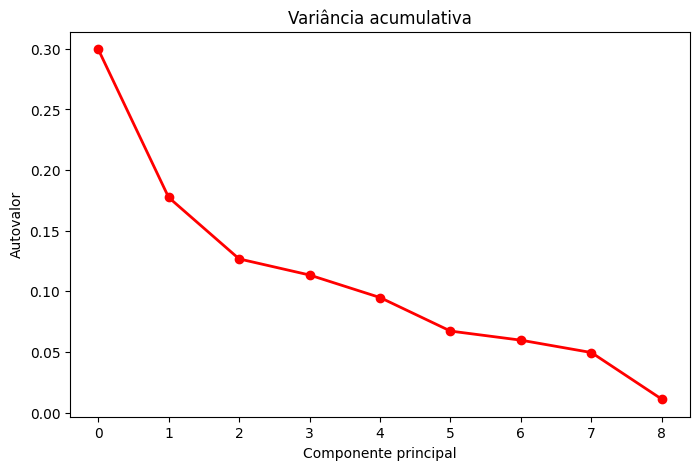
\includegraphics[scale=0.5]{img/acum.png}
    \caption{Visualização da variância acumulativa dos nove componentes.}
\end{figure}
É realizada a escolha e manutenção de um número específico de componentes principais obtidos pela Análise de Componentes Principais (PCA). O valor três é atribuido à variável n\_components que define quantas dessas componentes principais serão retidas para análises subsequentes. A escolha tem por objetivo facilitar a interpretação por meio de visualização gráfica em três dimensões. 
\subsection{Autovalores e autovetores}
\par São obtidos os autovalores e autovetores associados às componentes principais resultantes da aplicação da Análise de Componentes Principais (PCA). Os autovalores representam as variâncias explicadas por cada componente principal, enquanto os autovetores são os vetores próprios que indicam as direções das maiores variabilidades nos dados originais. \\
\begin{verbatim}
Autovalores (Variância Explicada por Componente Principal):
Componente Principal 1: 2.6975
Componente Principal 2: 1.5975
Componente Principal 3: 1.1414
...

Autovetores:
Componente Principal 1: [ 0.19902105  0.50868515  0.4642411   0.23032726 
0.16779264  0.32969422
  0.29940045 -0.3335565   0.30871732]
Componente Principal 2: [ 0.31164815 -0.2263488  -0.26758498  0.59527613 
0.58400529  0.01531499
  0.12540025  0.25789319 -0.04642641]
Componente Principal 3: [-0.31865865 -0.34919549 -0.37684689  0.01732992 
0.05903687 -0.01862812
  0.21461951 -0.48264747  0.59275863]
  ...
\end{verbatim}
\section{Visualização}
A partir dos dados obtidos na implementação, é criado um conjunto de visualizações com o intuito de possibilitar uma maior compreensão sobre os dados obtidos.\\
\subsection{Componentes principais}
\par A primeira visualização gerada foi o gráfico tridimensional das componentes principais obtidas pela Análise de Componentes Principais (PCA), colorindo os pontos de acordo com a presença ou ausência da Síndrome Metabólica. O mapa de cores personalizado utiliza a cor roxa para representar a classe 0 (ausência) e a cor laranja para a classe 1 (presença). A escolha dessas cores é estratégica para proporcionar uma representação visual clara e distintiva das duas classes.
\begin{figure}[htbp]
    \centering
    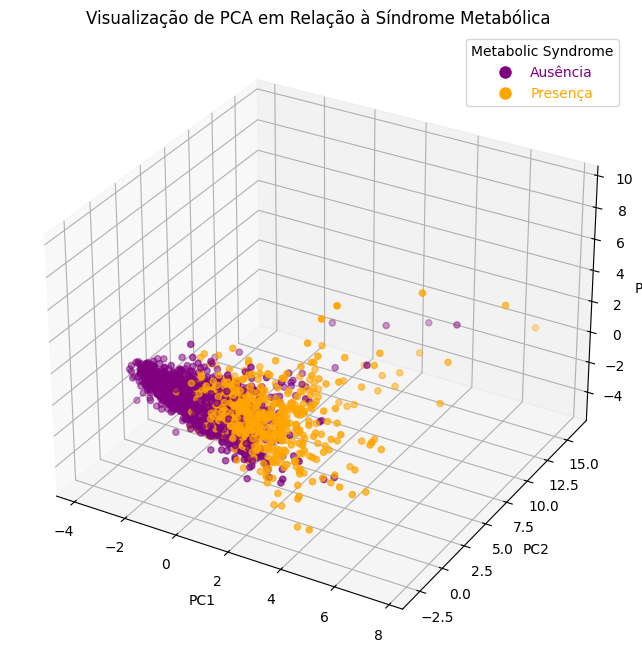
\includegraphics[scale=0.5]{img/pca_3d.png}
    \caption{Visualização do PCA em relação à Síndrome Metabólica.}
\end{figure}
\break

Com base na visualização do gráfico tridimensional gerado pela Análise de Componentes Principais (PCA), algumas observações podem ser inferidas:
\begin{itemize}
\item As duas nuvens de pontos, representando as classes "Ausência" e "Presença" da Síndrome Metabólica, estão predominantemente próximas, sugerindo que as amostras compartilham características semelhantes em termos das três primeiras componentes principais (PC1, PC2, e PC3).
\item Embora as nuvens estejam próximas, a um indício de que elas não se sobrepõem significativamente. Isso sugere que há uma pequena distinção entre as características representativas de cada classe nas primeiras três componentes principais.
\end{itemize} \\
\\
\par Utilizou-se a técnica de agrupamento K-Means aplicada às coordenadas das componentes principais separadamente para as classes "Ausência" e "Presença" da Síndrome Metabólica, para se obter outra perspectiva na distribuição dos dados. O intuito principal é realizar a clusterização das coordenadas das componentes principais para cada classe, identificando padrões ou grupos que possam indicar estruturas distintas nas representações das variáveis originais. Essa abordagem de agrupamento é valiosa para a caracterização mais detalhada das relações presentes nos dados. Para esse estudo, foram gerados oito clusters para a classe "Ausência" e oito para classe "Presença".

\begin{figure}[htbp]
    \centering
    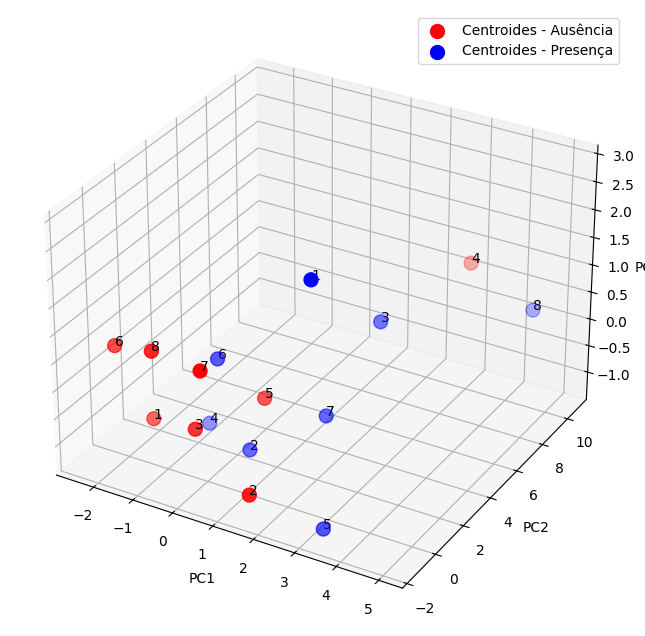
\includegraphics[scale=0.5]{img/k_mean.png}
    \caption{Visualização da clusterização dos dados do PCA.}
\end{figure}
\break

\par O resultado visual fornece insights sobre a estrutura subjacente dos dados e a eficácia do K-Means na identificação de padrões distintos nas representações de componentes principais. \\

\par Após a obtenção de clusters, são calculadas estatísticas descritivas para cada coordenadas das componentes principais, tanto para a classe "Ausência" quanto para a classe "Presença" da Síndrome Metabólica, com base nos centróides obtidos após a aplicação do algoritmo K-Means. Essas análises possibilitaram a criação de gráficos que informação sobre relações entre o PCA para cada classe.

\begin{figure}[htbp]
    \centering
    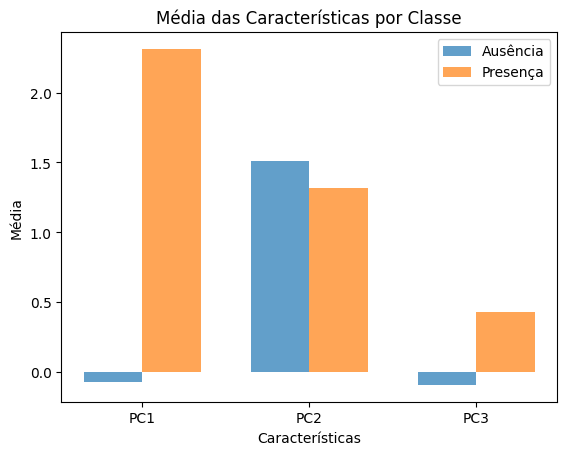
\includegraphics[scale=0.5]{img/k_media.png}
    \caption{Média das características por classe.}
\end{figure}
\begin{figure}[htbp]
    \centering
    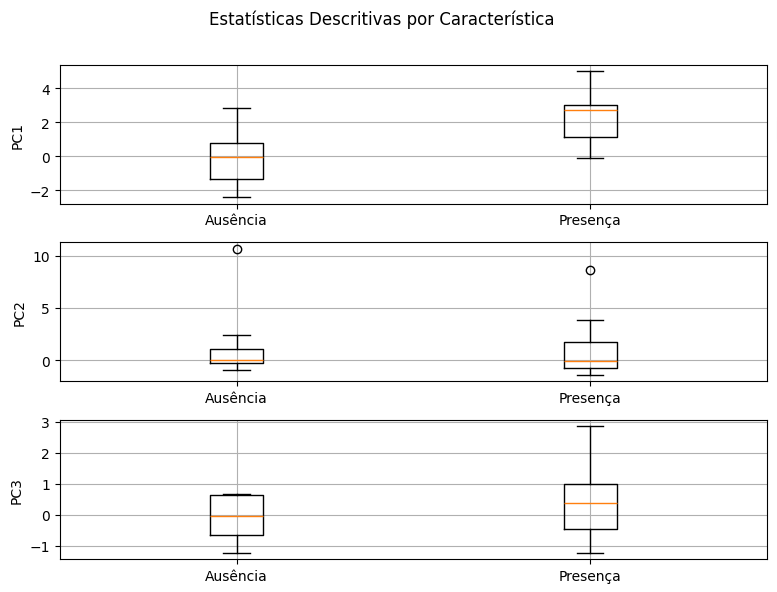
\includegraphics[scale=0.4]{img/est_carac.png}
    \caption{Estatísticas por característica e classe.}
\end{figure}
\break
\subsection{Análise de centróides de Clusters}
Ao analisar os centróides obtidos pelo K-Means para as classes de "Ausência" (Classe 0) e "Presença" (Classe 1), podemos extrair algumas conclusões preliminares sobre as tendências e padrões nas coordenadas das componentes principais (PCAs) associadas à Síndrome Metabólica baseando-se na análise estatística descritiva e visual realizada.

Para PC1 As amostras de "Presença" tendem a se posicionar mais nas coordenadas positivas, enquanto as amostras de "Ausência" têm uma distribuição mais equilibrada. Para PC2, Amostras de "Ausência" e "Presença" têm médias próximas, mas a variabilidade é mais alta em "Ausência". Para PC3 As amostras de "Presença" tendem a ter médias mais positivas e uma variabilidade um pouco maior em comparação com "Ausência".

\subsection{Decomposição em Valores Singulares}
A natureza dos dados possibilitou a aplicação da técnica de Decomposição em Valores Singulares (SVD, do inglês Singular Value Decomposition) à matriz de dados padronizados (X\_scaled). O SVD é uma técnica matemática fundamental que descompõe uma matriz em três componentes: a matriz de transformação à esquerda (U), a matriz diagonal contendo os valores singulares (Sigma), e a matriz de transformação à direita (Vt). Essa decomposição é uma ferramenta poderosa em análise de dados. Os resultados da decomposição estão visíveis no código disponíbilizado no repositório deste trabalho.

\section{Conclusão}

O estudo e aplicação da Análise de Componentes Principais (PCA) revelam-se fundamentais para a compreensão dos padrões subjacentes em conjuntos de dados multidimensionais. Ao longo da elaboração deste trabalho, explorando as nuances do cálculo das componentes principais e sua utilidade na identificação de estruturas complexas presentes nos dados. Os resultados obtidos, expressos através de gráficos, estatísticas descritivas e boxplots, proporcionam uma compreensão aprofundada das diferenças nas representações das classes "Ausência" e "Presença" da Síndrome Metabólica nas componentes principais presentes nos dados estudados. Essa análise sugere a presença de padrões distintos que merecem uma análise mais aprofundada. \\

\par Para facilitar o acesso e promover discussões adicionais sobre os resultados obtidos, o código completo encontra-se disponível no repositório
\begin{center}
\url{ https://github.com/neocrz/pca }
\end{center}
onde se encontram os dados originais, o arquivo latex 'main.tex' do presente texto, a implementação em código no documento 'pca.ipynb' que contém todas as análises e resultados.
\newpage
\printbibliography
\end{document}
